%=====================================================================
\chapter{Avaliação de usabilidade usando \aladim}
\label{usabilityEvaluation}
%=====================================================================

Avaliar a usabilidade  ainda em tempo de design  é uma alternativa que
pode reduzir os  custos de um projeto de  software.  A economia ocorre
por  permitir uma  entrega mais  rápida do  software e  evitar  que os
problemas  de  usabilidade apenas  sejam  corrigidos  após sessões  de
testes, o que  requer mudanças não só no código  da interface, mas até
mesmo   em  sua  arquitetura,   como  aponta~\citeonline{Folmer:2005}.
Avaliações em  tempo de projeto podem ocorrer,  de forma complementar,
tanto em  protótipos quanto em  modelos do software.   Neste capítulo,
busca-se  mostrar  como \aladim\  permite  a  realização de  avaliação
formativa,  através  da   inspeção  dos  modelos,  possibilitando  aos
avaliadores  identificar  problemas  nas  intenções  comunicativas  do
designer.

A avaliação de usabilidade pode abranger todo ciclo de desenvolvimento
e, segundo  \citeonline{Hix:1993}, ela  pode ser classificada  em {\em
  avaliação  formativa}  ou  {\em  avaliação somativa}.   A  avaliação
somativa é realizada sobre protótipos  de média ou alta fidelidade, ou
mesmo pelo  sistema já  implementado, o que  faz com que  os problemas
encontrados possam  acarretar altos custos de  reprojeto.  A avaliação
formativa,  foco  desta  proposta,  procura identificar  problemas  de
usabilidade logo  nos estágios iniciais do  projeto.  Vários artefatos
podem servir de  base para este tipo de  avaliação, entre eles podemos
destacar: cenários, modelos de  tarefa, modelos de diálogo/interação e
protótipos de baixa e média fidelidade~\cite{Hix:1993}.

%=====================================================================
\section{Inspeção de usabilidade em modelos}
\label{modelsInspection}
%=====================================================================

A  avaliação  da  usabilidade  foi  durante  muito  tempo  uma  tarefa
realizada apenas nas  fases de testes e implantação  dos sistemas.  Um
dos  problemas  desse  processo  é  que ele  exige,  tanto  o  sistema
funcionando,  quanto  um  conjunto  representativo de  seus  usuários.
Outro  problema, mais  crítico ainda,  é a  descoberta  tardia.  Pois,
segundo~\citeonline{Folmer:2004},  muitos   problemas  de  usabilidade
podem demandar mudanças significativas  em várias camadas do sistema e
não apenas na camada da interface.

Atualmente, cada vez mais profissionais  de \ihc\ têm buscado evitar a
descoberta tardia dos problemas  de usabilidade, procurando aplicar no
design   o  conhecimento   baseado   nas  experiências   profissionais
adquiridas  ao longo  dos anos.   Esses conhecimentos  são normalmente
concretizados sob a forma de princípios, diretrizes e padrões, visando
auxiliar o  designer na  melhoraria da qualidade  de uso  dos sistemas
interativos.

\citeonline[p.~320]{Dix:etal:2004}  defendem  que  é  vantajoso  fazer
avaliação ao longo do processo de design, além disso, argumentam que o
ideal seria  realizar a primeira avaliação antes  de qualquer trabalho
de implementação ter sido  iniciado.  Entretanto, eles argumentam que,
durante o design  pode ser custoso conduzir testes  com usuário, e que
podem existir  ainda, situações onde sua participação  não é possível.
Para isso,  eles destacam alguns  métodos de avaliação  realizados por
especialistas sem a necessidade da presença efetiva do usuário.  Entre
esses métodos está a {\em avaliação baseada em modelos}.

Nesse  tipo de avaliação,  \citeonline[p.~326]{Dix:etal:2004} destacam
que  o modelo  de diálogo  pode ser  usado para  avaliar  problemas de
usabilidade,  tais como  estados inalcançados,  diálogos  circulares e
complexidade de diálogos.  Possibilitando, dessa forma, a avaliação do
design  da  interação, antes  da  implementação  da interface.   Dessa
forma,  uma investigação sobre  avaliação de  usabilidade por  meio de
inspeção  de modelos de  interação é  justificada, quando  se pretende
identificar   problemas   de  usabilidade   nas   fases  iniciais   do
desenvolvimento.

%=====================================================================
\section{O método de inspeção \aladim}
\label{aladimInspection}
%=====================================================================

Buscando   antecipar  a  identificação   de  possíveis   problemas  de
usabilidade em sistemas interativos  desenvolvidos a partir de modelos
\aladim, definiu-se um método  de avaliação de usabilidade, baseado em
inspeção, cujas fases serão descritas na seção \ref{inspectionMethod}.
Considerando as  próprias limitações de  \aladim, o método é  capaz de
auxiliar  na  identificação de  um  número  limitado  de problemas  de
usabilidade.  Portanto,  é preciso  definir uma classificação  para os
tipos de problemas que o método é capaz de identificar.

Como um método subjetivo o  resultado da sua aplicação irá depender da
interpretação  do avaliador  durante a  inspeção do  modelo  usando as
diretrizes.   Mesmo  não  sendo   exigido  que  o  avaliador  seja  um
especialista  de \ihc,  é imprescindível  que possua  conhecimentos na
linguagem \aladim.  Além  disso, se feita por mais  de um avaliador, a
avaliação irá contribuir para  resultados mais precisos e um relatório
mais rico,  juntando todas as  análises subjetivas de  cada avaliador.
Dessa  forma,  é sugerido  que  um número  de  ímpar  (três podem  ser
suficientes)  de   avaliadores  para  evitar   possíveis  impasses  na
consolidação do relatório final.

\aladim\  oferece  uma  visão  abstrata  do processo  de  interação  e
navegação entre diferentes elementos da interface sem a necessidade de
tratar detalhes  de {\em layout}, cores e  outros elementos estéticos.
Dessa forma,  um método de  inspeção nos modelos \aladim\  não permite
que  problemas   de  usabilidade,  associados  a   esses  aspectos  de
apresentação,  sejam  identificados.   Nesse sentido,  definiu-se  uma
classificação  dos tipos  de problemas  que são  possíveis identificar
durante a inspeção em modelos \aladim, usando o método proposto.

Esta  classificação está  baseada  em fundamentos  já consolidados  na
literatura  sobre problemas  de  usabilidade. Isto  é, cada  categoria
considera os tipos de  problemas identificados pelas {\em heurísticas}
de  \citeonline{Nielsen:1994}   e  pelas  {\em  regras   de  ouro}  de
\citeonline{Shneiderman:1998}.  A descrição  das categorias, a seguir,
referencia as respectivas fundamentações, nos trabalhos citados, sendo
{\em H} para as heurísticas e {\em RO} para as regras de ouro:

\begin{enumerate}
  \renewcommand{\labelenumi}{$C_{\arabic{enumi}}$}

  \item {\em Problemas relacionados  à falta de visibilidade do estado
    do sistema} ($H_5$ e $RO_3$). A interface de um sistema interativo
    deve manter  o usuário informado  daquilo que ele está  fazendo em
    prazo razoável, indicando que  entendeu sua solicitação e que está
    realizando o processamento necessário para atendê-la.  Pretende-se
    identificar antecipadamente  os erros desta  categoria nos modelos
    \aladim,  através  da   diretrizes  $D_{1}$,  $D_{2}$,  $D_{3}$  e
    $D_{4}$.

  \item {\em  Problemas relacionados à falta de  controle explícito do
    usuário} ($H_6$ e $RO_7$). O  sistema não pode obrigar o usuário a
    permanecer numa situação indesejada,  ele deve permitir ao usuário
    decidir sobre suas próprias ações, como agente ativo na interação.
    Pretende-se identificar  antecipadamente os erros  desta categoria
    nos  modelos  \aladim,  através  da diretrizes  $D_{5}$,  $D_{6}$,
    $D_{7}$ e $D_{8}$.

  \item  {\em  Problemas  relacionados  à  falta  de  consistência  do
    diálogo} ($H_1$ e $RO_4$). As sequências de ações do usuário sobre
    a interface  devem ser  organizadas de maneira  natural, indicando
    que elas possuem início,  meio e fim, deixando claro especialmente
    quando elas terminam.   Pretende-se identificar antecipadamente os
    erros desta  categoria nos modelos \aladim,  através da diretrizes
    $D_{9}$, $D_{10}$ e $D_{11}$.

  \item {\em Problemas relacionados à falta de prevenção e recuperação
    de erros} ($H_9$  e $RO_5$). O sistema deve  prevenir o usuário de
    cometer  erros, mas  se isso  ocorrer, deve  auxiliá-lo oferecendo
    instruções  simples,  construtivas   e  específicas  para  ele  se
    recuperar.  Pretende-se identificar antecipadamente os erros desta
    categoria  nos modelos  \aladim, através  da  diretrizes $D_{12}$,
    $D_{13}$ e $D_{14}$.

\end{enumerate}

%=====================================================================
\subsection{Diretrizes para inspeção}
\label{inspectionGuidelines}
%=====================================================================

A partir da  classificação dos problemas de usabilidade  que podem ser
identificados, definiu-se  um conjunto de  diretrizes, cujas violações
indiquem que  a interface  pode levar o  usuário a  experimentar algum
tipo  de  problemas  de  usabilidade  daquela  categoria  associada  à
diretriz  violada.  Vale  ressaltar que  \aladim\ representa  apenas a
interação,  não sendo  possível  avaliar aspectos  de apresentação  da
interface  (layout, tipos  de widgets,  etc), o  que  inviabiliza, por
exemplo,   a   avaliação   de   aspectos   estéticos   da   interface.
Inicialmente, o conjunto definido  é composto por quatorze diretrizes,
descritas         a        seguir        e         resumidas        na
tabela~\ref{tab:inspectionGuidelines},  de acordo com  a classificação
da seção~\ref{aladimInspection}.

\begin{table}[!htb]
  \small
  \begin{center}

    \begin{tabular}{|c|m{145mm}|} \hline

      \multicolumn{2}{|l|}{\bf  $C_1$  --   Relacionados  à  falta  de
        visibilidade do estado do sistema} \\ \hline

      $D_{1}$  &  Um  espaço  de interação  sincronizado  deve  conter
      interações básicas  informando o estado da  função da aplicação.
      \\ \hline

      $D_{2}$ & Um  espaço de interação que recebe  informações de uma
      função da aplicação  deve conter interações básicas apresentando
      esses resultados. \\ \hline

      $D_{3}$ & Um espaço de  interação que compõe uma sequência, deve
      conter  interações  básicas  informando  qual o  passo  atual  e
      quantos restam.  \\ \hline

      $D_{4}$  & Um  espaço  de  interação que  aciona  uma função  da
      aplicação  que resulta em  alterações irreversíveis  deve conter
      interações básicas solicitando confirmação.  \\ \hline
     
      \multicolumn{2}{|l|}{\bf  $C_2$  --   Relacionados  à  falta  de
        controle explícito do usuário} \\ \hline

      $D_{5}$  &  Um  espaço  de interação  sincronizado  deve  conter
      interações básicas que possibilitem  o cancelamento da função da
      aplicação.  \\ \hline

      $D_{6}$ &  Um espaço  de interação decorrente  de uma  reação de
      fracasso deve conter interações  básicas que permitam ao usuário
      sair daquele estado indesejado. \\ \hline

      $D_{7}$  & Um espaço  de interação  interno numa  sequência deve
      conter  interações básicas  que  permitam ao  usuário voltar  ao
      espaço de interação anterior. \\ \hline

      $D_{8}$  & Um  espaço  de  interação que  aciona  uma função  da
      aplicação  que resulta em  alterações irreversíveis  deve conter
      interações básicas solicitando confirmação. \\ \hline

      \multicolumn{2}{|l|}{\bf  $C_3$  --   Relacionados  à  falta  de
        consistência do diálogo} \\ \hline

      $D_{9}$ &  Um espaço de interação deve  conter apenas interações
      básicas relevantes ao  contexto da funcionalidade controlada por
      ele. \\ \hline

      $D_{10}$ & Um espaço de interação deve conter interações básicas
      associadas  a  expressões  e  conceitos familiares  ao  usuário.
      \\ \hline
   
      $D_{11}$  & Um  espaço  de interação  que  possui uma  interação
      básica, que ativa uma  navegação para outro espaço de interação,
      deve possuir  nomenclatura correlata  ao espaço de  interação de
      destino.  \\ \hline

      \multicolumn{2}{|l|}{\bf  $C_4$  --   Relacionados  à  falta  de
        prevenção e recuperação de erros} \\ \hline

      $D_{12}$ & Em um espaço de interação decorrente de uma reação de
      fracasso  devem   existir  interações  básicas   que  apresentem
      mensagens de erro de forma clara para o usuário. \\ \hline

      $D_{13}$ &  Um espaço de  interação que exige tomada  de decisão
      sobre caminhos  alternativos deve conter  interações básicas que
      auxiliem o usuário nessa decisão. \\ \hline

      $D_{14}$ &  Quando passível de  falha durante sua  execução, uma
      função de  aplicação deve  possuir reações de  falha transitando
      para   espaços   de   interação   que  informem   claramente   o
      problema. \\ \hline

    \end{tabular}
    \caption{Resumo das diretrizes de inspeção para modelos \aladim.}
    \label{tab:inspectionGuidelines}
  \end{center}
\end{table}

\begin{enumerate}
  \renewcommand{\labelenumi}{$D_{\arabic{enumi}}$}

%%   $C_1$  --  Relacionados à  falta  de  visibilidade  do estado  do
%%   sistema

  \item  {\em   Um  espaço  de  interação   sincronizado  deve  conter
    interações básicas  informando o  estado da função  da aplicação}.
    Se o  diagrama possuir algum  espaço de interação  sincronizado, o
    inspetor   deve  verificar  se   ele  possui   interações  básicas
    informando  do processamento e  de seu  progresso, do  contrário o
    usuário não irá perceber isso  e poderá achar que o sistema travou
    ou não iniciou o processamento.

  \item  {\em Um  espaço de  interação que  recebe informações  de uma
    função  da aplicação deve  conter interações  básicas apresentando
    esses resultados}.   O inspetor deve  verificar se esse  espaço de
    interação  traz  interações básicas  apresentando  o resultado  do
    processamento  executado pelo  sistema.  Do  contrário,  o sistema
    perde seu propósito de atender o usuário em suas solicitações.

  \item {\em  Um espaço  de interação que  compõe uma  sequência, deve
    conter interações básicas informando  qual o passo atual e quantos
    restam}. O  inspetor deve identificar uma sequência  de espaços de
    interação e verificar se estes informam ao usuário em que ponto da
    sequência  ele está  atuando  e quantos  faltam  para finalizar  a
    sequência e assim, alcançar seu objetivo.

  \item {\em Um espaço de interação que aciona uma função da aplicação
    cujas  pré-condições não estão  satisfeitas deve  condicionar suas
    interações básicas de acionamento}.  O inspetor deve verificar se,
    para  uma função  de  aplicação que  demandar  o preenchimento  de
    determinadas  informações  por  parte  do  usuário,  o  espaço  de
    interação condicionou a interação  básica de ativação da função às
    outras  interações   básicas  usadas  para   o  preenchimento  das
    informações,  que  poderá  ser  feita através  da  condições  e/ou
    operadores.
     
%%  $C_2$ -- Relacionados à falta de controle explícito do usuário

  \item  {\em   Um  espaço  de  interação   sincronizado  deve  conter
    interações básicas  que possibilitem  o cancelamento da  função da
    aplicação}. O inspetor deve identificar quais espaços de interação
    estão sincronizados com alguma  função de aplicação e verificar se
    eles  possuem interações  básicas  que permitam  ao usuário,  caso
    deseje, cancelar  a execução da  função da aplicação  sem prejuízo
    para o estado da aplicação e consistência das informações.

  \item  {\em Um  espaço  de  interação decorrente  de  uma reação  de
    fracasso deve  conter interações  básicas que permitam  ao usuário
    sair  daquele estado  indesejado}.  O  propósito de  um  espaço de
    interação  resultado  de uma  reação  de  fracasso,  é auxiliar  o
    usuário no  entendimento do problema  ocorrido e, se  possível, na
    resolução do  mesmo. Para  isso, o inspetor  dever verificar  se o
    espaço de interação possui  as interações básicas necessárias para
    apresentar as informações  sobre o problema e indicar  o que fazer
    para sair daquele estado.

  \item  {\em Um  espaço de  interação interno  em uma  sequência deve
    conter interações básicas que permitam ao usuário voltar ao espaço
    de interação anterior}. O  inspetor deve identificar os espaços de
    interação  dentro de  uma sequência  e verificar,  se a  partir do
    primeiro,  cada  um  deles  possui  alguma  interação  básica  que
    possibilite ao  usuário, caso deseje, voltar ao  passo anterior da
    sequência.

  \item {\em Um espaço de interação que aciona uma função da aplicação
    que  resulta em  alterações irreversíveis  deve  conter interações
    básicas solicitando confirmação}. O  inspetor deve verificar se há
    interações  básicas informando  ao usuário  sobre  suas alterações
    permanentes sobre  o estado do sistema,  especialmente aquelas que
    resultam na remoção/exclusão de informações.
     
%%  $C_3$ -- Relacionados à falta de consistência do diálogo

  \item  {\em Um  espaço de  interação deve  conter  apenas interações
    básicas  relevantes ao contexto  da funcionalidade  controlada por
    ele}.   O inspetor  deve verificar  se em  um espaço  de interação
    possui  interações  básicas,  não  relacionadas  à  funcionalidade
    associada, que possam concorrer com o foco de atenção do usuário.

  \item  {\em Um espaço  de interação  deve conter  interações básicas
    associadas  a expressões  e conceitos  familiares ao  usuário}.  O
    inspetor  deve   verificar  se  há   interações  básicas  contendo
    elementos conceituais que não sejam do domínio no usuário.
   
  \item {\em  Um espaço de  interação que possui uma  interação básica
    que  ativa  uma navegação  para  outro  espaço  de interação  deve
    possuir nomenclatura correlata ao espaço de interação de destino}.
    O  inspetor deve  verificar  se informação  associada à  interação
    básica  de  ativação  da   navegação,  reflete  o  que  o  usuário
    irá/poderá fazer no espaço de interação de destino.

%%     Exemplo:  {\tt activate  ``Cadastrar  cliente''}, ativando  uma
%%     navegação  para um  espaço de  interação chamado  ``Consulta de
%%     cliente''.

%%  $C_4$ -- Relacionados à falta de prevenção e recuperação de erros

  \item {\em  Em um  espaço de interação  decorrente de uma  reação de
    fracasso devem existir interações básicas que apresentem mensagens
    de  erro  de  forma  clara  para  o  usuário}.   O  inspetor  deve
    identificar esses espaços interação  e verificar se não são usadas
    interações básicas  apenas com informações  codificadas, ou apenas
    com termos técnicos, sobre os erros ocorridos.
    
  \item {\em Um espaço de  interação que exige tomada de decisão sobre
    caminhos alternativos deve  conter interações básicas que auxiliem
    o usuário  nesta decisão}. O inspetor deve  identificar os espaços
    de  interação  que  dividem  o  fluxo  da  interação  em  caminhos
    alternativos e  verificar se há interações  básicas informando dos
    diferentes caminhos e os possíveis resultados de cada um.

  \item {\em Quando passível de falha durante sua execução, uma função
    de  aplicação  deve  possuir  reações de  falha  transitando  para
    espaços  de  interação que  informem  claramente  o problema}.   O
    inspetor deve identificar essas  funções de aplicações e verificar
    se existem  transições do  tipo reações de  falha para  espaços de
    interação destinados a informar e auxiliar o usuário na solução do
    problema.

\end{enumerate}

Com  o objetivo  de exemplificar  o uso  das diretrizes  no  método, a
figura~\ref{fig:InspectionExemple} apresenta um  modelo de interação e
a respectiva lista de verificação, preenchida por um avaliador durante
a fase de  {\em coleta de dados}. Na figura é  possível perceber que o
avaliador considerou  que para o primeiro espaço  de interação, apenas
$D_{14}$ foi violada, $D_4$,  $D_9$ e $D_{10}$ estavam em conformidade
e as demais não eram aplicáveis. Enquanto que para o segundo espaço de
interação  $D_5$ e  $D_{13}$  foram violadas,  $D_1$,  $D_2$, $D_9$  e
$D_{10}$ estavam em conformidade e as demais não eram aplicáveis.

\begin{figure}[!htb]
  \begin{center}

    \subfigure[Modelo de interação]{
      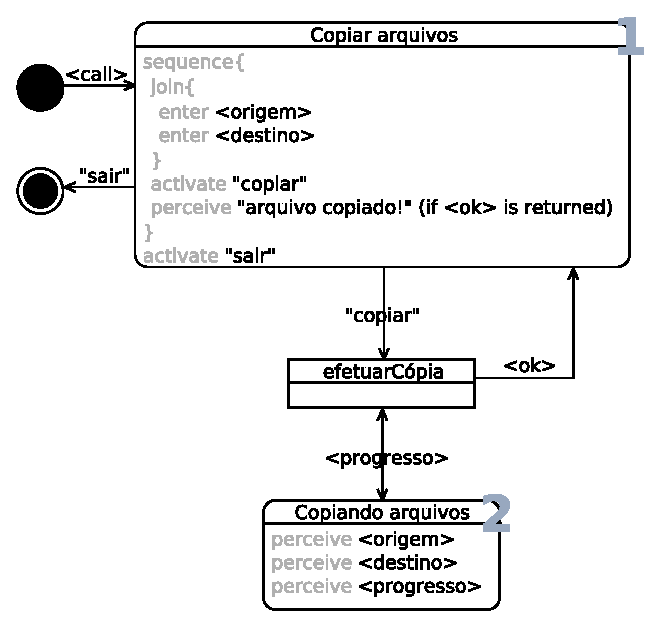
\includegraphics[scale=0.700]{images/copiarModel.eps}
    }\hspace{10mm}
    \subfigure[Lista de verificação]{
      \small
      \begin{tabular}[b]{|c|c|c|} \hline
        \multirow{2}{*}{\bf Diretriz} & 
        \multicolumn{2}{c|}{\bf Espaço de Interação} \\ \cline{2-3}

        & ~~~~~{\bf 1}~~~~~ & ~~~~~{\bf 2}~~~~~ \\ \hline

        $D_{1}$ & \na & \cf \\ \hline
        $D_{2}$ & \na & \cf \\ \hline
        $D_{3}$ & \na & \na \\ \hline
        $D_{4}$ & \cf & \na \\ \hline
        $D_{5}$ & \na & \vi \\ \hline
        $D_{6}$ & \na & \na \\ \hline
        $D_{7}$ & \na & \na \\ \hline
        $D_{8}$ & \na & \na \\ \hline
        $D_{9}$ & \cf & \cf \\ \hline
        $D_{10}$ & \cf & \cf \\ \hline
        $D_{11}$ & \na & \na \\ \hline
        $D_{12}$ & \na & \na \\ \hline
        $D_{13}$ & \cf & \na \\ \hline
        $D_{14}$ & \vi & \na \\ \hline
      \end{tabular}
    }
    \caption{Exemplo de coleta de dados feita por um avaliador durante
      a coleta de dados.}
    \label{fig:InspectionExemple}
  \end{center}
\end{figure}

A partir da  análise da figura~\ref{fig:InspectionExemple}, é possível
fazer  algumas  considerações,   sobre  dois  possíveis  problemas  de
usabilidade que poderão ser  concretizados na interface, caso ela seja
implementada com base nesse modelo de interação.  O primeiro refere-se
um  potencial  problema  relacionado  {\em  à  falta  de  prevenção  e
  recuperação  de  erros}  (categoria  $C_4$),  isso  que  porque,  se
acontecer  alguma falha  na execução  do processo  de cópia,  não está
designado  um local  onde o  usuário possa  receber  alguma informação
sobre o  problema, o que é  antecipado com a violação  de $D_{14}$, no
primeiro espaço de  interação, pois a função da  aplicação associada a
ele,  pode falhar  e não  há reações  de falha  para nenhum  espaço de
interação.

O segundo potencial problema está relacionado {\em à falta de controle
  explícito do usuário} (categoria  $C_2$), isso porque, se o usuário,
mesmo  acompanhando o  progresso  da execução  do  processo de  cópia,
julgar que  vai demorar mais do  que ele está disposto  a esperar, ele
não poderá cancelar o processo e terá obrigatoriamente que esperar até
sua conclusão, o que é antecipado  com a violação de $D_5$, no segundo
espaço de interação.

%=====================================================================
\subsection{Fases do método inspeção}
\label{inspectionMethod}
%=====================================================================

Como  se  conhece  na  literatura,  métodos  de  inspeção,  como  {\em
  avaliação     heurística}~\cite{Nielsen:1994},     {\em     percurso
  cognitivo}~\cite{Wharton:etal:1994}       e       {\em      inspeção
  semiótica}~\cite{deSouza:etal:2006} são constituídos por um conjunto
de passos ou  fases que visam instruir o  avaliador durante o processo
de  execução do  método  para  obter os  resultados  esperados em  sua
aplicação. De modo  semelhante, o método de inspeção  proposto para os
modelos \aladim, é constituído de três fases, descritas a seguir:

\begin{enumerate}

  \item  {\em  Preparação}:  Nesta  fase, os  avaliadores  preparam  o
    material usado na avaliação,  que, essencialmente, são: os modelos
    de  interação e as  fichas com  a lista  de verificação  para cada
    modelo   a   ser   inspecionado.   Contudo,   adicionalmente,   os
    avaliadores podem lançar mão dos documentos sobre os requisitos do
    sistema  para  auxiliá-los  no  entendimento sobre  o  domínio  da
    aplicação sendo avaliada.

  \item {\em  Coleta e  interpretação dos dados}:  Esta é uma  fase de
    execução  individual,  onde cada  avaliador  irá inspecionar  cada
    modelo   e  preencher   sua  respectiva   lista   de  verificação,
    atribuindo,  para  cada  espaço  de interação,  sua  avaliação  da
    diretriz, indicando  um dos seguintes  valores: {\em Conformidade}
    (\cf),  {\em Violação}  (\vi) e  {\em  Não se  aplica} (\na).   Na
    sequência,   cada   avaliador   cria   sua  lista   de   problemas
    identificados,   indicando   seu   local,  sua   severidade,   sua
    justificativa e alguma recomendação de solução.

  \item {\em Consolidação e relato dos resultados}: Esta última fase é
    de   execução  coletiva,   onde  todos   os   avaliadores  revisam
    conjuntamente suas listas  de problemas, julgando suas respectivas
    relevâncias,   severidades,    justificativas   e   recomendações.
    Finalmente,  produzem  um  relatório  consolidado,  descrevendo  o
    processo de  inspeção e  os resultados obtidos,  ou seja,  a lista
    definitiva dos problemas identificados.

\end{enumerate}

Alguns pontos precisam ser  esclarecidos sobre o processo de inspeção.
O  primeiro diz  respeito  ao fato  dos  textos da  descrição de  cada
diretriz serem  orientados aos espaços de interação.   O que significa
que as diretrizes devem ser verificadas ou confrontadas aos espaços de
interação.  Excepcionalmente, $D_{14}$  possui texto baseado na função
da aplicação.  Contudo, o avaliador  deve aplicar a diretriz ao espaço
de interação que aciona a função da aplicação, visto que, este seria o
último espaço de interação com o qual o usuário teria interagido antes
da   falha    ocorrer.    Isto   foi   demostrado    no   exemplo   da
figura~\ref{fig:InspectionExemple},  como pode  ser percebido,  que os
espaços de  interação fora enumerados  e distribuídos na tabela  com a
lista de verificação.

Considerando que a  lista de verificação tem duas  dimensões, uma para
os  espaços de  interação  e  outra para  as  diretrizes, o  avaliador
poderá,  estrategicamente, fixar  uma  diretriz e  percorrer todos  os
espaços  de interação,  ou fixar  um espaço  de interação  e percorrer
todas as diretrizes.  Por conveniência,  poderá se formatar a lista de
verificação  de  maneira   tabular,  estabelecendo,  por  exemplo,  as
diretrizes ao longo das linhas e  os espaços de interação ao longo das
colunas,    o    que    também     foi    feito    no    exemplo    da
figura~\ref{fig:InspectionExemple}.

O  segundo  aspecto  diz  respeito  ao  julgamento  da  severidade  do
problema.  Por  isso, optou-se por  permitir que o avaliador  faça uso
das abordagens propostas  por \citeonline{Nielsen:1993}, que podem ser
uma {\em escala  de classificação simples}, com valores  lineares ou a
{\em  combinação das  dimensões} associadas  ao problema.   No  que se
refere  a uma  simples  escala,  pode-se ter  os  seguintes valores  e
significados~\cite[p.~103]{Nielsen:1993}:

\begin{enumerate}[start=0]

  \item {\em isto não é, de todo, um problema de usabilidade};

  \item {\em  problema cosmético}: não  precisa ser corrigido  a menos
    que haja tempo sobrando no projeto;

  \item {\em  problema de pequena importância}: a  correção deste tipo
    de problema deve ter baixa prioridade;

  \item {\em  problema de  grande importância}: é  importante corrigir
    este  problema,  portanto,  à  sua  correção deve  ser  dada  alta
    prioridade;

  \item  {\em  problema  catastrófico}:  é  imperativo  corrigir  este
    problema antes que o produto sendo avaliado possa ser liberado;
\end{enumerate}

Ainda  é possível  usar a  abordagem  da combinação  das dimensões  do
problema,  sugeridas  por  \citeonline[p.~104]{Nielsen:1993},  onde  o
avaliador poderá considerar, por exemplo, as seguintes dimensões:

\begin{itemize}

  \item  {\em frequência}:  indica qual  a proporção  de  usuários que
    experimentaram o problema;

  \item {\em impacto}: indica qual  o dano causado pelo problema sobre
    as atividades realizadas pelo usuário que experimentou o problema;

  \item  {\em persistência}:  indica se  o problema  ocorre  apenas na
    primeira vez  que o usuário interage  com o sistema e  não mais se
    repete após superado,  ou continuará se repetindo persistentemente
    sempre que o usuário interagir com o sistema.

\end{itemize}

Vale   ressaltar   que   a    adoção   da   abordagem   proposta   por
\citeonline[p.~103-104]{Nielsen:1993}    para   a    identificação   e
tratamento da severidade dos  erros de usabilidade encontrados durante
a inspeção \aladim,  segue integralmente a proposta de  forma que mais
detalhes e exemplos podem ser obtidos diretamente na documentação.

%=====================================================================
\section{Experimento de validação do método}
\label{evaluation}
%=====================================================================

Com o objetivo de validar o método de inspeção \aladim, realizou-se um
estudo experimental,  que consistiu na inspeção de  um modelo \aladim,
usando  as diretrizes  definidas  na seção~\ref{inspectionGuidelines},
visando  a identificação  de problemas  de usabilidade.   O  modelo de
interação utilizado resultou da  engenharia reversa da interface usada
para realização de uma tarefa, na agência virtual de um banco estatal.

Os resultados  das inspeções foram  confrontados aos resultados  de um
teste de usabilidade executado  na referida interface, que serviram de
gabarito,   confirmando  se   determinado   problema  de   usabilidade
identificado durante a inspeção  do modelo foi, de fato, experimentado
pelo usuário, durante o teste de usabilidade.  A seguir, é apresentado
o {\em gabarito} e como seu  deu sua construção, bem como a definição,
o planejamento, a execução, a  operação, validação dos dados e análise
\&   interpretação   do    experimento,   nos   moldes   da   proposta
\citeonline{Wohlin:etal:2000},    para    engenharia    de    software
experimental.

%=====================================================================
\subsection{Construção do gabarito}
\label{initialExperiments}
%=====================================================================

Como será definido na seção~\ref{studyGoal}, o experimento comparou os
resultados   da   inspeção   em   modelos   \aladim,   com   problemas
comprovadamente  já experimentados  pelos usuários,  durante o  uso do
sistema  objeto  de  inspeção  no experimento.   Esse  {\em  gabarito}
resulta dos dados de um teste de usabilidade previamente executado por
\citeonline{CostaNeto:etal:2011},  cuja  descrição  e  resultados  são
resumidos a seguir.

O   teste   envolveu   cinco   participantes,  todos   estudantes   de
pós-graduação e com  uma média de três anos de  experiência no uso dos
serviços do banco.   Cada sessão de teste foi  composta de duas fases.
A  primeira consistiu  das orientações  de como  seriam  realizados os
testes.  A segunda consistiu da atuação do usuário no uso do sistema e
respondendo  às  perguntas  realizadas  pelos  avaliadores  durante  a
interação.

Considerando que, atualmente, a maioria dos bancos oferece serviços de
{\it internet bank} aos seus  clientes e que não é incomum reclamações
de usuários que encontram algum tipo de dificuldade em utilizar alguns
desses serviços.   No referido trabalho,  o teste avaliou a  tarefa de
{\em adesão ao serviço de envio de mensagens SMS}, oferecido pela {\it
  Caixa Econômica Federal}, cujo cenário é descrito a seguir.

\begin{citacao}

  O cenário começa quando um cliente, na página principal, seleciona a
  opção  {\em  Mensagem  via  celular  - SMS},  então  o  sistema  lhe
  apresenta uma  breve explicação sobre  o serviço e  disponibiliza ao
  cliente  duas opções:  {\em  Excluir} e  {\em  Incluir}.  O  cliente
  seleciona  a  opção  {\em  Incluir},  depois disso,  o  sistema  lhe
  apresenta informações mais detalhadas sobre o serviço e mais algumas
  opções, dentre  elas a opção de {\em  Continuar}.  Selecionando {\em
    Continuar}, é  apresentado ao cliente  o {\em Termo de  Adesão} no
  qual ele tem a opção de {\em Concordar}.  Após marcar essa intenção,
  o  sistema solicita  os dados  sobre o  número do  telefone  que irá
  receber as mensagens  e a faixa de valores  das transações e oferece
  ao cliente  a opção  {\em Cadastrar}.  Após  o usuário  pressionar o
  botão {\em  Cadastrar}, o sistema  apresenta as informações  sobre a
  adesão e  solicita a  senha da  conta, o cliente  informa a  senha e
  seleciona {\em Confirmar}, o sistema  então informa ao cliente que a
  conta já está cadastrada~\cite[p.~128]{CostaNeto:etal:2011}.

\end{citacao}

Como  forma  de identificar  se  o  diálogo  apresentado pelo  sistema
avaliado possibilitava uma sequência  clara de interações, sob o ponto
de  vista do  usuário,  foram elaboradas  algumas  questões que  foram
aplicadas durante  a interação.  Estas  questões tinham o  objetivo de
conhecer o pensamento  do usuário e eram solicitadas  a cada página da
interface  apresentada durante  a observação  do sistema  em  uso. São
elas:

\begin{enumerate}
  \renewcommand{\labelenumi}{\alph{enumi})}

  \item Você consegue identificar onde está? Porque?
  \item O que você acha que pode/deve fazer agora? Porque?
  \item O que você acha que o sistema vai fazer a partir dessas ações?
    Porque?
\end{enumerate} 

É importante  ressaltar que nas intervenções  feitas pelos avaliadores
foram realizadas de  forma a não interferir na  experiência de uso dos
participantes,  ou seja,  limitou-se  apenas a  ouvir  e registrar  as
respostas  dadas  para  cada   questão.   Desta  forma,  foi  possível
identificar quais fatores ou problemas de usabilidade não permitiam ao
usuário saber, através  da interação, qual o estado  atual do sistema,
as possíveis ações que ele  podia executar e quais seriam os possíveis
efeitos destas ações.   Cada sessão de teste foi  registrada em áudio,
vídeo e  formulários, que foram  usados para coletar as  respostas dos
usuários às questões acima.  Estes registros foram produzidos usando a
ferramenta      {\em      RecordMyDesktop}\footnote{Disponível      em
  http://recordmydesktop.sourceforge.net}.

A  partir  da  lista  de  problemas encontrados  durante  o  teste  de
usabilidade, associou-se  cada problema  encontrado a uma  diretriz do
método de  inspeção, indicando que  o problema teria sido  causado por
sua  violação,  o  que  resultou  na  tabela~\ref{tab:testeProblemas}.
Também  foram indicadas as  diretrizes que  estavam em  conformidade e
quais não  se aplicavam aos  problemas encontrados.  Esse  processo de
associação,  produziu  a  lista   de  verificação  que  foi  usada  na
comparação   com  os   resultados  das   inspeções   realizadas  pelos
participantes         do         experimento,         feita         na
tabela~\ref{tab:DiretrizesFrequencia}, da  apresentação da estatística
descrita do experimento (seção~\ref{descriptiveStatistics}).

% Tabela dos problemas encontrados durante os testes de usabilidade
\begin{table}[!htb]
  \small
  \begin{center}
    \begin{tabular}{|c|m{76mm}|m{48mm}|c|} \hline

      {\bf \#} & {\bf Descrição} & {\bf Local/Página} & {\bf Violação}
      \\ \hline

      1 & O usuário não sabia em que ponto da tarefa estava.  & {\em 1
        - Selecionar conta} & $D_{3}$ \\ \hline

      2 & O usuário se questiona se incluir é a mesma coisa que aderir
      ao serviço.  & {\em 1 - Selecionar conta} & $D_{10}$ \\ \hline

      3 & O usuário se questiona  se já tivesse aderido e possuísse um
      telefone registrado.   & {\em 1  - Selecionar conta}  & $D_{13}$
      \\ \hline

      4 & O usuário não sabia em  que ponto da tarefa estava. & {\em 2
        - Apresentação do serviço} & $D_{3}$ \\ \hline

      5 & O usuário não sabia em que ponto da tarefa estava.  & {\em 3
        - Termo de adesão} & $D_{3}$ \\ \hline

      6 & O  usuário pretende voltar à página  anterior, mas o sistema
      não permitiu.  & {\em 3 - Termo de adesão} & $D_{7}$ \\ \hline

      7 & O  participante é levado à página  de {\em Selecionar conta}
      (início do cenário) ao clicar  no botão {\em Discordo}. & {\em 3
        - Termo de adesão} & $D_{11}$ \\ \hline

      8 & O participante se confunde sobre que ponto da tarefa está de
      fato. & {\em 4 - Dados para adesão} & $D_{3}$ \\ \hline

      9 & O  usuário pretende voltar à página  anterior, mas o sistema
      não permitiu.  & {\em 4 - Dados para adesão} & $D_{7}$ \\ \hline

      10 & O participante é  levado à página de {\em Selecionar conta}
      (inicio do cenário) ao clicar no botão {\em Retornar}.  & {\em 4
        - Dados para adesão} & $D_{11}$ \\ \hline

      11 & O  participante se confunde sobre que  ponto da tarefa está
      de fato.  & {\em 5 - Confirmação dos dados} & $D_{3}$ \\ \hline

      12 & O usuário pretende  voltar à página anterior, mas o sistema
      não  permitiu. &  {\em  5  - Confirmação  dos  dados} &  $D_{7}$
      \\ \hline

      13 & O participante é  levado à página de {\em Selecionar conta}
      (inicio do cenário) ao clicar no botão {\em Cancelar}.  & {\em 5
        - Confirmação dos dados} & $D_{11}$ \\ \hline

      14 & O usuário pretende  voltar à página anterior, mas o sistema
      não  permitiu.   & {\em  5  -  Conta  já cadastrada}  &  $D_{7}$
      \\ \hline

      15 & O participante é  levado à página de {\em Selecionar conta}
      (inicio do cenário) ao clicar no botão {\em Voltar}.  & {\em 5 -
        Conta já cadastrada} & $D_{11}$ \\ \hline

    \end{tabular}
    \caption{Problemas encontrados durante o teste de usabilidade.}
    \label{tab:testeProblemas}
  \end{center}
\end{table}

%=====================================================================
\subsection{Definição do experimento}
\label{experimentDefining}
%=====================================================================

De acordo com \citeonline{Wohlin:etal:2000}, é nesta fase que ocorre a
concepção  do experimento, através  da definição  de quais  os objetos
serão estudados, quais os  propósitos do estudo, quais características
dos objetos serão estudas,  sob quais perspectivas os resultados serão
interpretados e em  qual ambiente o estudo irá  ocorrer.  Dessa forma,
considerando         o          guia         prático,         proposto
por~\citeonline{Solingen:Berghout:1999}   para  aplicação   do  método
\gqm\ ({\em \Gqm}) de~\citeonline{Basili:etal:1994}, são apresentados,
a seguir, o objetivo, as questões e as métricas deste experimento.

%=====================================================================
\subsubsection{Objetivo}
\label{studyGoal}
%=====================================================================

Considerando          o          esquema         proposto          por
\citeonline[p.~51]{Solingen:Berghout:1999}, este  estudo visa analisar
           {\em  o  método de  inspeção  de  modelos  \aladim}, com  o
           propósito  de  {\em   caracterizar}  a  sua  capacidade  de
           identificação antecipada  de problemas de  usabilidade, com
           respeito à  sua {\em  eficácia}, em comparação  à avaliação
           feita sobre  o sistema em uso,  do ponto de  vista dos {\em
             avaliadores   de  usabilidade},   no  contexto   do  {\em
             desenvolvimento de sistemas interativos}.

%=====================================================================
\subsubsection{Questões}
\label{studyQuestions}
%=====================================================================

Visando alcançar o objetivo estabelecido acima e considerando o método
proposto  por  \citeonline{Solingen:Berghout:1999},  este  experimento
busca responder as seguintes questões:

\begin{enumerate}
  \renewcommand{\labelenumi}{$Q_{\arabic{enumi}}$}

  \item A  inspeção permitiu identificar os  problemas apresentados no
    gabarito, isto é, que foram encontrados em ambas as avaliações?

  \item A inspeção identificou  problemas que não estavam no gabarito,
    isto é, não foram encontrados apenas na inspeção?

  \item A inspeção não identificou problemas apresentados no gabarito,
    isto é, que foram encontrados apenas no teste de usabilidade?

  \item  O  método  de  inspeção,  usando  o  conjunto  de  diretrizes
    apresentado, foi considerado aceitável pelos participantes?

\end{enumerate}

%=====================================================================
\subsubsection{Métricas}
\label{studyMetrics}
%=====================================================================

Para responder às questões da seção~\ref{studyQuestions}, é necessário
estabelecer algumas  métricas. Para as três primeiras  questões, o que
se  pretende medir,  são  os problemas  identificados  na inspeção  em
comparação  com  os problemas  encontrados  no  teste de  usabilidade.
Contudo,  cada  problema  encontrado   no  teste  de  usabilidade  foi
associado a  uma das diretrizes  do método de inspeção,  produzindo um
gabarito  com uma  lista de  verificação das  diretrizes  violadas, em
conformidade  e  não  aplicadas, vide  seção~\ref{initialExperiments}.

Dessa forma,  o que se precisa  medir são os números  de diretrizes em
conformidade, violadas  e não aplicadas  do gabarito em  comparação às
listas  de  verificação  preenchidas  pelos participantes  durante  as
sessões de inspeção. Por isso, optou-se por fazer uso de uma matriz de
confusão~\cite{Tan:etal:2005}, apresentada na tabela~\ref{tab:matriz},
onde  as linhas  representam a  {\em classe  real}  (classificação das
diretrizes feita durante as inspeções) e as colunas representam a {\em
  classe predita} (classificação das diretrizes no gabarito).  Onde os
valores representam, respectivamente: {\bf 1} -- Conformidade, {\bf 2}
-- Violação,  {\bf 3}  --  Não se  aplica.   Portanto, empregou-se  as
seguintes métricas para as respectivas questões:

\begin{enumerate}

  \renewcommand{\labelenumi}{$Q_{\arabic{enumi}}$}

  \item Esta questão foi medida pelo número de problemas identificados
    na inspeção e  que constavam no gabarito do  teste de usabilidade,
    isto é,  onde as diretrizes  foram violadas nas duas  situações, o
    que corresponde aos elementos $f_{22}$ da matriz de confusão.

  \item Esta questão foi medida pelo número de problemas identificados
    na inspeção mas não constavam no gabarito do teste de usabilidade,
    isto  é, onde  as diretrizes  estavam  em conformidade  ou não  se
    aplicavam no teste de usabilidade, o que corresponde aos elementos
    $f_{21}$ e $f_{23}$ da matriz de confusão.

  \item Esta questão foi medida pelo número de problemas que constavam
    no gabarito do teste, mas que não foram identificados na inspeção,
    isto  é onde  as  diretrizes  estavam em  conformidade  ou não  se
    aplicavam na inspeção, o  que corresponde aos elementos $f_{12}$ e
    $f_{32}$ da matriz de confusão.

  \item Esta questão foi medida  pela análise dos dados produzidos por
    uma      adaptação      do      formulário      SUS,      proposto
    por~\citeonline{Brooke:1996}.

\end{enumerate}

\begin{table}[!htb]
 \begin{center}
   \begin{tabular}{|c|c|c|c|c|} \cline{3-5}
     \multicolumn{2}{c|}{} &
     \multicolumn{3}{c|}{\bf Gabarito} \\ \cline {3-5}

     \multicolumn{2}{c|}{} & 
     {\bf \cf~~(1)} & {\bf \vi~~(2)} & {\bf \na~~(3)}  \\ \hline

     \multirow{3}{*}{\bf Inspeção} & {\bf \cf~~(1)} & 

%     \cellcolor{blue!25}
     $f_{11}$ & $f_{12}$ & $f_{13}$ \\ \cline{2-5}

     & {\bf \vi~~(2)} & 
     $f_{21}$ & $f_{22}$ & $f_{23}$ \\ \cline{2-5}

     & {\bf \na~~(3)} & 
     $f_{31}$ & $f_{32}$ & $f_{33}$ \\ \hline

   \end{tabular}
   \caption{Matriz           de           confusão,           adaptada
     de~\citeonline[p.~169]{Tan:etal:2005}.}
   \label{tab:matriz}
 \end{center}
\end{table}

%=====================================================================
\subsection{Planejamento}
\label{planning}
%=====================================================================

Segundo  \citeonline{Wohlin:etal:2000}, esta fase  é composta  de sete
atividades,  a seleção  do  contexto, a  formulação  das hipóteses,  a
seleção  de  variáveis,  a  seleção  dos participantes,  o  modelo  do
experimento,  a instrumentação  e  a avaliação  de  validade, que  são
apresentadas a seguir.

%=====================================================================
\subsubsection{Seleção do contexto}
\label{contextSelection}
%=====================================================================

Esta  atividade visa caracterizar  o contexto  onde o  experimento foi
realizado. Segundo  \citeonline{Wohlin:etal:2000}, esta caracterização
deve cobrir as seguintes dimensões:

\begin{itemize}

  \item {\em Processo}: o experimento não foi executado em um processo
    formal de  desenvolvimento de software, ou seja,  foi executado em
    um processo {\em off-line};

  \item {\em  Participantes}: o experimento não foi  executado por uma
    equipe de profissionais, mas por uma equipe de {\em estudantes} da
    área de computação;

  \item  {\em  Realidade}:  o  experimento  endereçou  problemas  {\em
    reais}, encontrados na agência virtual de um banco;

  \item {\em  Generalidade}: o  experimento não pode  ser generalizado
    por  ser válido  apenas  para o  contexto  {\em específico}  deste
    estudo.

\end{itemize}

%=====================================================================
\subsubsection{Definição das hipóteses}
\label{hypothesisFormulation}
%=====================================================================

O principal fundamento para análise  estatística de um experimento é o
teste  de  hipótese.  Para  isso,  uma  ou  mais hipóteses  devem  ser
formuladas, deixando  claro o que se pretende  avaliar no experimento.
Buscando avaliar  o grau de  concordância entre as  classificações das
diretrizes,  no  gabarito  e  nas  inspeções,  foi  empregado  o  {\em
  Coeficiente Kappa},  proposto por~\citeonline{Cohen:1960} e definido
pela  equação~\ref{eq:Kappa}.  Sendo  que este  experimento  partiu da
hipótese que  há concordância entre a classificação  das diretrizes no
gabarito e  nas inspeções.  Dessa forma, as  seguintes hipóteses foram
consideradas:

\begin{itemize}

  \item {\em Nula}: não há concordância entre a classificação feita no
    teste e a classificação feita na inspeção, ou seja $H_0$: $k = 0$.

  \item   {\em   Alternativa}:   há   alguma  concordância   entre   a
    classificação feita no teste  e a classificação feita na inspeção,
    ou seja, $H_1$: $k > 0$

\end{itemize}

\begin{equation}
  k = \frac{p_{o} - p_{e}}{1 - p_{e}}
  \label{eq:Kappa}
\end{equation}

\begin{tabular}{cl}
  sendo: & 
  $p_{o} = \frac{acertos}
  {acertos + erros}$ \\
  & $p_{e} = \displaystyle\sum_{i=1}^{n}(p_{i1} \times p_{i2})$
\end{tabular}

\begin{tabular}{ll}
  onde: 

  & $acertos=$ soma  dos elementos da diagonal principal  da matriz de
  confusão\\

  & $erros=$ soma  dos elementos fora da diagonal  principal da matriz
  de confusão\\

  & $n =$ número de categorias\\
  & $i =$ número da categoria (de $1$ até $n$)\\

  &  $p_{i1} =$  proporção  de  ocorrência da  categoria  $i$ no  {\em
    gabarito}\\

  &  $p_{i2} =$  proporção  de  ocorrência da  categoria  $i$ na  {\em
    inspeção}

\end{tabular}

%=====================================================================
\subsubsection{Seleção de variáveis}
\label{variablesSelection}
%=====================================================================

Nesta   fase,   foram   selecionadas   as  variáveis   dependentes   e
independentes,  que  representam,  respectivamente  as entradas  e  os
resultados  do  processo  de  experimentação.  Neste  experimento,  as
variáveis definidas foram as seguintes:

\begin{itemize}

  \item {\em Independentes} (entradas): o modelo de interação descrito
    em \aladim\ e a lista de verificação usados na inspeção e gabarito
    resultante do teste usado na comparação;

  \item {\em Dependentes} (resultados):  as listas de verificações com
    as  classificações  das  diretrizes  nas  inspeções e  o  grau  de
    concordância entre inspeção e gabarito na comparação;

\end{itemize}

%=====================================================================
\subsubsection{Seleção dos participantes}
\label{subjectsSelection}
%=====================================================================

A  abordagem   escolhida  para  a  seleção   dos  participantes  deste
experimento  é feita  por  conveniência, ou  seja, foram  selecionados
dezenove alunos  da disciplina {\em Projeto de  Interface de Usuário},
dos  cursos  de graduação  em  {\em  Engenharia  de Software}  e  {\em
  Ciências da Computação}, da  {\em Universidade Federal do Rio Grande
  do Norte}.

%=====================================================================
\subsubsection{Modelo do experimento}
\label{experimentDesign}
%=====================================================================

Apesar deste  experimento procurar comparar o  resultado das inspeções
com o resultado previamente  estabelecido, seu modelo experimental foi
considerado      do      tipo       ``um      fator      com      dois
tratamentos''~\cite[p.~54]{Wohlin:etal:2000}, que foram definidos como
entradas  ou variáveis  independentes. Mesmo  o resultado  do primeiro
tratamento  (considerado aqui,  o teste  de usabilidade)  já  ter sido
produzido, buscou-se garantir os seguintes princípios:

\begin{itemize}

  \item {\em Aleatorização}: Neste experimento, todos os participantes
    aplicaram o  mesmo tratamento (inspeção)  sobre o mesmo  objeto ao
    mesmo tempo,  dessa maneira, não foi  preciso aleatorizar qualquer
    ordem na execução dos testes.

  \item  {\em  Bloqueio}: Neste  experimento  não foram  identificados
    fatores  que  pudessem   causar  efeitos  indesejáveis,  dadas  as
    condições de execução dos testes. Contudo, diante da possibilidade
    de  não saber o  quanto os  participantes aprenderam  \aladim, bem
    como o  entendimento das diretrizes,  considerou-se eliminar dados
    que  estivessem longe  da  média  geral da  turma,  como visto  na
    seção~\ref{operationValidation}.

  \item   {\em  Balanceamento}:   Neste  experimento,   não   houve  a
    necessidade  de   se  realizar  o  balanceamento,   visto  que  os
    participantes   tinham  o  mesmo   perfil,  receberem   as  mesmas
    informações  sobre  o  método  de  inspeção e  aplicaram  o  mesmo
    tratamento ao mesmo objeto e ao mesmo tempo.

\end{itemize}

%=====================================================================
\subsubsection{Instrumentação}
\label{experimentInstrumentation}
%=====================================================================

Consiste  da descrição  dos instrumentos  que foram  usados  durante a
execução      dos       testes      do      experimento.       Segundo
\citeonline{Wohlin:etal:2000}, os  instrumentos são de  três tipos: os
objetos, as  guias e as medições.   Neste experimento, o  objeto foi o
modelo de  interação, usando a  linguagem \aladim, produzido  a partir
das  interfaces do  sistema avaliado,  para a  mesma  tarefa realizada
durante o teste de usabilidade (seção~\ref{initialExperiments}), que é
apresentado na figura~\ref{fig:CookieModel}.

\figura{Modelo de interação inspecionada durante o experimento.}
       {fig:CookieModel}
       {cookieModel.eps}
       {0.700}
       {-90}

Para  guiar  os  participantes  no experimento,  os  mesmos  receberam
treinamento na linguagem \aladim, bem como esclarecimentos sobre o uso
das  diretrizes,  visto  que  cada teste  experimental  (aplicação  do
tratamento  ao  objeto   pelo  participante)  consistiu  da  atividade
inspeção do modelo \aladim.   Além disso, para realização da inspeção,
os  participantes  seguiram  a  {\em  lista  de  verificação}  com  as
diretrizes.

As  medições  foram realizadas  por  meio  da  coleta de  informações,
durante  as  sessões  de  teste  experimental,  inspeção.   Assim,  os
problemas de usabilidade identificados foram medidos por meio das {\em
  listas de  verificações}, já o  perfil dos participantes  foi medido
por meio do questionário pré-teste, enquanto que a aceitação do método
foi medida  por meio de  questionário pós-teste, que consistiu  de uma
adaptação do formulário SUS proposto por \citeonline{Brooke:1996}.

%% Todos  os  instrumentos usados  no  experimento,  são apresentados  no
%% apêndice~\ref{} deste documento.

%=====================================================================
\subsubsection{Avaliação da validade}
\label{validityEvaluation}
%=====================================================================

Consiste em  assegurar que  os resultados produzidos  pelo experimento
sejam válidos, no mínimo para a amostra da população que foi submetida
aos testes. Como os resultados  dos testes de usabilidade foram usados
como gabarito, assume-se a validade mínima do mesmo, sobre sua amostra
de participantes.  Assim, considerando os tipos de validades definidos
por \citeonline{Wohlin:etal:2000}, neste experimento, eles foram assim
avaliados:

\begin{itemize}

  \item {\em  Conclusão}: Com a  finalidade de se  realizar conclusões
    válidas sobre  o experimento, foi usado o  {\em Coeficiente Kappa}
    (seção~\ref{hypothesisFormulation})   para   medir   o   grau   de
    concordância entre  as classificações  das diretrizes em  ambas as
    avaliações.   Para uma  boa  compreensão do  grau de  concordância
    foram        usadas       as        interpretações       sugeridas
    por~\citeonline{Landis:Koch:1977}.

  \item  {\em Interna}:  Os participantes  executaram  suas inspeções,
    individualmente, para que nenhum tivesse influência de outro.

  \item {\em Construção}:  Por se tratar de um  método de avaliação de
    usabilidade, foi usada a  quantidade de problemas encontrados, por
    ser  um importante  indicador  de produtividade  do método.   Além
    disso,  foi  usado  o  formulário  SUS que  possui  seus  próprios
    indicadores de  confiança das respostas  coletadas.  Como apontado
    no trabalho  de~\citeonline{Tullis:Stetson:2004}, ele apresentou o
    melhor  percentual   de  conclusões  corretas,   sobre  os  demais
    estudados, em amostras superiores a oito indivíduos.

  \item  {\em Externa}:  Apesar  de não  se  pretender generalizar  as
    conclusões deste experimento,  todos os participantes selecionados
    possuíam  o perfil  adequado, assim  como  o ambiente  e o  tempo,
    necessários para sua execução, também foram adequados.

\end{itemize}

%=====================================================================
\subsection{Operação}
\label{operation}
%=====================================================================

Após  definido   e  planejado,  o   experimento  foi  operacionalmente
conduzido  de maneira que  se pode  coletar os  dados, posteriormente,
analisados.    Segundo  \citeonline{Wohlin:etal:2000},  esta   fase  é
constituída dos passos de preparação, execução e validação dos dados.

%=====================================================================
\subsubsection{Preparação}
\label{operationPrepartation}
%=====================================================================

A todos  os participantes foram dados esclarecimentos,  sobre todos os
aspectos  étnicos  envolvidos  na  participação  de  cada  um.   Foram
garantidos, o anonimato e  a possibilidade de desistir da participação
a  qualquer momento.   Os questionários  pré e  pós-teste, bem  como a
lista   de  verificação   necessários   à  coleta   dos  dados   foram
disponibilizados.

%=====================================================================
\subsubsection{Execução}
\label{operationExecution}
%=====================================================================

Imediatamente antes da  seção de testes, o moderador  expôs o que cada
participante deveria executar,  explicando as diretrizes e demostrando
um exemplo  de como preencher a  lista de verificação, a  partir de um
modelo  usado  para  esta   finalidade.   Durante  toda  a  sessão  de
inspeções,  o moderador  ficou  à disposição  para esclarecer  dúvidas
eventuais.   A coleta  de dados  foi feita  pelo  próprio participante
através  do  preenchimento dos  questionários  pré  e  pós-teste e  do
preenchimento do {\em lista de verificação}.

%=====================================================================
\subsubsection{Validação dos dados}
\label{operationValidation}
%=====================================================================

Foram  eliminados   da  análise,   os  dados  dos   participantes  que
preencheram erroneamente quaisquer dos  materiais de coleta. Em função
da aplicação dos testes experimentais, terem ocorridos em sala de aula
com participação de todos os  alunos da turma, também foram eliminados
os dados  dos alunos que não  participaram da seção  de treinamento na
linguagem \aladim, bem como na aplicação das diretrizes.

A partir  das médias  de diretrizes em  conformidades, violadas  e não
aplicadas,  foi  observado  que   os  dados  de  alguns  participantes
encontravam-se  distante dessas  médias.  Dessa  forma,  optou-se pela
{\em  média truncada  ou podada},  calculada a  partir da  remoção dos
dados de dois participantes, um  de cada extremo, ficando para análise
os dados de dezessete participantes.

Para  o preenchimento do  questionário pós-teste,  dois participantes,
por algum motivo não identificado, não preencherem o formulário SUS, o
que  reduziu  os  dados  deste  formulário para  um  total  de  quinze
participantes.

%=====================================================================
\subsection{Análise e interpretação}
\label{analysis}
%=====================================================================

Após a  coleta e  validação dos dados  produzidos na fase  de operação
(seção~\ref{operation}),    estes   precisaram   ser    analisados   e
interpretados.  Esta  fase é  constituída pelos passos  de estatística
descritiva e teste de hipótese, apresentados a seguir.

%=====================================================================
\subsubsection{Estatística descritiva}
\label{descriptiveStatistics}
%=====================================================================

Aqui busca-se descrever e  representar graficamente vários aspectos de
interesse sobre  os dados.  Entre  os aspectos incluem-se  medidas que
indiquem, por exemplo, como alguma escala está posicionada no conjunto
de dados,  bem como o quanto  o conjunto de dados  está concentrado ou
espalhado.  Dessa  forma, pode-se  obter algumas medidas  de tendência
central e dispersão, como mediana, mínimos e máximos.

No  que se  refere ao  quantitativo de  diretrizes e  suas categorias,
apresentado   na   figura~\ref{fig:DiretrizesSumario},  foi   possível
observar as  medidas para classificação das  diretrizes nas categorias
conformidade, violação e não se aplica foram, respectivamente, mediana
de 8, 4 e 1, com máximos de 11, 8 e 5 e mínimos de 5, 1 e 0.

\figura{Sumário da classificação das diretrizes.}
       {fig:DiretrizesSumario}
       {diretrizesSumario.eps}
       {0.850}
       {0}

No  que se  refere  à distribuição  da  classificação das  diretrizes,
representada  na  figura~\ref{fig:DiretrizesFrequencia}, foi  possível
observar que  algumas diretrizes foram  classificadas numa determinada
categoria  por mais de  $^2/_3$ dos  participantes, como  é o  caso da
categoria  de  {\em  Conformidade}.   Enquanto outras,  não  foram  em
determinada categoria por  nenhum dos participantes, como é  o caso da
categoria {\em Não se aplica}.

\figura{Frequência de distribuição de avaliação das diretrizes.}
       {fig:DiretrizesFrequencia}
       {diretrizesFrequencia.eps}
       {0.750}
       {0}

Vale ressaltar  que a classificação  de cada diretriz  foi determinada
pela       categoria        de       maior       frequência.        Na
tabela~\ref{tab:DiretrizesFrequencia}, são  apresentados os resultados
de classificação feita no gabarito  e nas inspeções do modelo \aladim,
sendo  que esta  foi determinada  pela maior  frequência  relativa, ou
seja, a  classificação que foi definida pela  maioria dos avaliadores,
acompanhada da  respectiva frequência.  Para  caso de empate  entre as
maiores  frequências,  o desempate  seguiu  uma  ordem de  prioridade,
estabelecida entre  as categorias, que  foi {\em violação}  sobre {\em
  conformidade} e {\em conformidade} sobre {\em não se aplica}.

Com  as listas  de verificação  com as  classificações  resultantes do
teste    de   usabilidade   e    das   inspeções,    apresentadas   na
tabela~\ref{tab:DiretrizesFrequencia},  procedeu-se  a  construção  da
matriz de confusão (tabela~\ref{tab:matrizResultado}), onde nas linhas
estão  as  classificações  obtidas  nas  inspeções e  nas  colunas  as
classificações preditas (gabarito) que  foram obtidas durante o teste.
A partir  dos números  obtidos na matriz  de confusão e  dos problemas
associados  às diretrizes  violadas (tabela~\ref{tab:testeProblemas}),
foram  estabelecidas as  métricas  (seção~\ref{studyMetrics}), com  as
quais foi possível  responder às questões (seção~\ref{studyQuestions})
do experimento, conforme descrições a seguir.

\begin{table}[!htb]
  \begin{center}

     \begin{tabular}{|c|c|c|c|} \hline
      {\bf Diretriz} & {\bf Gabarito} &{\bf Inspeção} & {\bf Frequência} \\ \hline

      $D_{1}$  & \na & \na & 47,06\% \\ \hline % 3
      $D_{2}$  & \cf & \cf & 76,47\% \\ \hline % 1
      $D_{3}$  & \vi & \cf & 47,06\% \\ \hline % 1
      $D_{4}$  & \cf & \cf & 52,94\% \\ \hline % 1
      $D_{5}$  & \na & \na & 41,18\% \\ \hline % 3
      $D_{6}$  & \na & \cf & 88,24\% \\ \hline % 1
      $D_{7}$  & \vi & \vi & 47,06\% \\ \hline % 2
      $D_{8}$  & \na & \vi & 47,06\% \\ \hline % 2
      $D_{9}$  & \cf & \cf & 82,35\% \\ \hline % 1
      $D_{10}$ & \vi & \cf & 82,35\% \\ \hline % 1
      $D_{11}$ & \vi & \vi & 47,06\% \\ \hline % 2
      $D_{12}$ & \cf & \cf & 94,12\% \\ \hline % 1
      $D_{13}$ & \vi & \vi & 47,06\% \\ \hline % 2
      $D_{14}$ & \cf & \cf & 76,47\% \\ \hline % 1
    \end{tabular}
    \caption{Classificação das diretrizes no teste e na inspeção.}
    \label{tab:DiretrizesFrequencia}
  \end{center}
\end{table}

Métrica  associada  à questão  $Q_1$,  que  é  o número  de  problemas
identificados  em ambas  avaliações.  Considerando  que as  {\em três}
diretrizes  classificadas como  violadas tanto  no gabarito  quanto na
inspeção  (elementos $f_{22}$  da matriz  de confusão)  foram $D_{7}$,
$D_{11}$  e  $D_{13}$ e  que  elas  estavam  associadas a  {\em  nove}
problemas de  usabilidade, é  possível afirmar que  {\bf sim},  a {\em
  inspeção  sobre  modelos  identificou  problemas  que  foram  também
  encontrados no teste de usabilidade}.

Métrica  associada  à questão  $Q_2$,  que  é  o número  de  problemas
identificados  durante a inspeção,  mas que  não foram  encontrados no
teste.    Considerando   que  a   diretriz   classificada  como   {\em
  conformidade}  ou   {\em  não  se   aplica}  no  gabarito   mas  foi
classificada como  {\em violada}  pela inspeção (elementos  $f_{21}$ e
$f_{23}$  da matriz  de confusão)  foi $D_{8}$  e que  ela  não estava
associada a nenhum dos problemas  presentes no teste de usabilidade, é
possível  afirmar   que  {\bf  sim},  a   {\em  inspeção  identificou,
  erroneamente, problemas que  não foram experimentados pelos usuários
  durante o teste}.

\begin{table}[!htb]
 \begin{center}

   \begin{tabular}{|c|c|c|c|c|} \cline{3-5}
     \multicolumn{2}{c|}{} &
     \multicolumn{3}{c|}{\bf Gabarito} \\ \cline {3-5}

     \multicolumn{2}{c|}{} & 
     {\bf \cf~~(1)} & {\bf \vi~~(2)} & {\bf \na~~(3)}  \\ \hline

     \multirow{3}{*}{\bf Inspeção} & {\bf \cf~~~(1)} & 

     5 & 2 & 1 \\ \cline{2-5}

     & {\bf \vi~~(2)} & 
     0 & 3 & 1 \\ \cline{2-5}

     & {\bf \na~~~(3)} & 
     0 & 0 & 2 \\ \hline

   \end{tabular}
   \caption{Matriz de confusão para avaliação final do experimento.}
   \label{tab:matrizResultado}
 \end{center}
\end{table}

Métrica associada  à questão  $Q_3$, que é  o número de  problemas que
foram  encontrados  no  teste,  mas  que não  foram  identificados  na
inspeção. Considerando que as {\em duas} diretrizes classificadas como
violadas no gabarito, mas que foram classificadas como conformidade ou
não se aplica na inspeção  (elementos $f_{12}$ e $f_{32}$ da matriz de
confusão) foram  $D_{3}$ e  $D_{10}$ e que  elas estavam  associadas a
{\em seis} problemas de usabilidade, é possível afirmar que {\bf sim},
a  {\em  inspeção  de  modelos  não identificou  problemas  que  foram
  encontrados durante o teste}.

Para  responder a  questão  $Q_4$, verificou-se  o  grau de  aceitação
medido pelo formulário SUS.  \citeonline[p.192]{Brooke:1996} apresenta
o  procedimento  para  se  calcular  o  grau  de  aceitação  usando  o
questionário.    Os  valores  obtidos   para  cada   participante  são
apresentados na figura~\ref{fig:SusResultados}.   Onde, os dados foram
sumarizados com  o mínimo de  45, máximo de  82,5 e mediana  de 68,75.
Considerando que  o grau de aceitação  médio da turma foi  de 66,88 e,
também,              considerando              o              trabalho
de~\citeonline[p.~118]{Bangor:etal:2009}, pode-se  concluir que o grau
de aceitação  médio foi considerado satisfatório por  ficar entre {\em
  OK} (50,9) e {\em Good} (71,4).

\begin{figure}[!htb]
  \begin{center}

    \subfigure[Valores do grau de aceitação]{
      \small
      \begin{tabular}[b]{|c|c|c|c|} \hline
        {\bf \#} & {\bf Idade} & 
        {\bf Sexo} & {\bf Grau} (SUS) \\ \hline

        $p_{1}$ & 24 & Masculino & 77,50 \\ \hline
        $p_{2}$ & 19 & Feminino & 72,50 \\ \hline
        $p_{3}$ & 21 & Masculino & 82,50 \\ \hline
        $p_{4}$ & 19 & Masculino & 57,50 \\ \hline
        $p_{5}$ & 20 & Masculino & 67,50 \\ \hline
        $p_{6}$ & 23 & Masculino & 77,50 \\ \hline
        $p_{7}$ & 21 & Feminino & 75,00 \\ \hline
        $p_{8}$ & 20 & Masculino & 60,00 \\ \hline
        $p_{9}$ & 20 & Masculino & 70,00 \\ \hline
        $p_{10}$ & 20 & Masculino & 45,00 \\ \hline
        $p_{11}$ & 28 & Masculino & 62,50 \\ \hline
        $p_{12}$ & 19 & Masculino & 55,00 \\ \hline
        $p_{13}$ & 21 & Masculino & 67,50 \\ \hline
        $p_{14}$ & 18 & Feminino & 55,00 \\ \hline
        $p_{15}$ & 23 & Masculino & 72,50 \\ \hline
      \end{tabular}

    }\hspace{10mm}
    \subfigure[Sumário dos graus de aceitação]{
      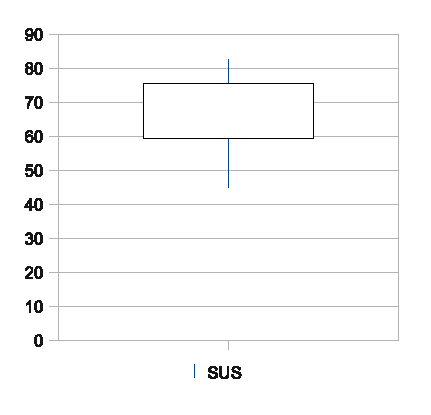
\includegraphics[scale=0.700]{images/aceitacaoSumario.eps}
    }
    \caption{Resultados do formulário SUS.}
    \label{fig:SusResultados}
  \end{center}
\end{figure}

%=====================================================================
\subsubsection{Teste estatístico ou teste de hipótese}
\label{hypothesisTest}
%=====================================================================

Considerando que $H_0: k = 0$,  isto é, a hipótese depende do valor de
$k$,  a  primeira  coisa  a   se  fazer  foi  realizar  o  cálculo  do
coeficiente,    cuja    fórmula    de    cálculo   foi    dada    pela
equação~\ref{eq:Kappa},                 apresentada                 na
seção~\ref{hypothesisFormulation}.   Assim,  seguem  os  cálculos  dos
elementos:

\begin{displaymath}
  p_{o} = 
  \frac{acertos}{acertos + erros} =
  \frac{10}{10 + 4} = 0,7143
\end{displaymath}

\begin{displaymath}
  p_{e} = 
  \displaystyle\sum_{i=1}^{n}(p_{i1} \times p_{i2}) = 
  \left(\frac{5}{14} \times \frac{8}{14}\right) + 
  \left(\frac{5}{14} \times \frac{4}{14}\right) + 
  \left(\frac{4}{14} \times \frac{2}{14}\right) = 0,3469
\end{displaymath}

\begin{displaymath}
  k = \frac{p_{o} - p_{e}}{1 - p_{e}} =
  \frac{0,7143 - 0,3469}{1 - 0,3469} = 0,5625
\end{displaymath}

O valor do coeficiente  é imprescindível para validação dos resultados
do experimento. Contudo, é importante entender o que significa o valor
do  coeficiente obtido,  ou seja,  se o  resultado representa  uma boa
concordância ou não.  Para isso, \citeonline{Landis:Koch:1977} propõem
uma  classificação  desse  valor, atribuindo-lhe  interpretações  mais
descritivas  para  cinco  intervalos,   como  pode  ser  observado  na
tabela~\ref{tab:Agreement}.

\begin{table}[!htb]
 \begin{center}

   \begin{tabular}{cl} \hline

     {\bf Valor de $k$} & {\bf Concordância} \\ \hline
      $<0,00$     & Insignificante \\
      $0,00-0,20$ & Leve \\ 
      $0,21-0,40$ & Razoável \\ 
      $0,41-0,60$ & Moderada \\ 
      $0,61-0,80$ & Substancial \\ 
      $0,81-1,00$ & Quase perfeita \\ \hline

   \end{tabular}
   \caption{Interpretações        para        o        valor        do
     coeficiente~\cite[p.~165]{Landis:Koch:1977}.}
   \label{tab:Agreement}
 \end{center}
\end{table}

A partir do valor de  $k$, procedeu-se aplicação do teste estatístico,
que  foi o  {\em teste  mono-caudal à  direita}, cujos  resultados são
apresentados na  tabela~\ref{tab:Teste}.  Considerando que  o valor de
$k$, obtido, foi  0,5625 e que o valor de P  foi de 0,0020 ($P<0,05$),
com  intervalo de  confiança (95\%)  entre  0,2001 e  0,9249, o  teste
estatístico permitiu que a hipótese nula fosse {\bf rejeitada}.

\begin{table}[!htb]
  \begin{center}

    \begin{tabular}{|m{37mm}|m{20mm}|} \hline
      Coeficiente Kappa & 0,5625 \\ \hline
      $z$                 & 2,8876 \\ \hline
      P                   & 0,0019 \\ \hline
      Intervalo de confiança (95\%)~$\alpha=0,05$ & 
      {\em sup}: 0,9249 {\em inf}:~~~0,2001 \\ \hline
    \end{tabular}
    \caption{Resultado do teste estatístico.}
    \label{tab:Teste}
  \end{center}
\end{table}

%=====================================================================
\section{Considerações sobre o experimento}
\label{inspectionClosures}
%=====================================================================

O  experimento  consistiu  da  realização  da inspeção  de  um  modelo
\aladim, usando  as diretrizes do método  e com o  objetivo de apontar
potenciais problemas de  usabilidade presentes no processo interativo.
O  modelo  utilizado  representa  um  cenário de  uso  de  um  sistema
existente.    Os  resultados  desta   etapa  foram   confrontados  aos
resultados de um teste de  usabilidade executado na interface do mesmo
sistema,  que serviram  de  {\em gabarito}.   Após  isso, uma  análise
estatística  permitiu   verificar  se  os   problemas  de  usabilidade
identificados   durante   as   inspeções   do  modelo   foram   também
identificados nos testes com usuários.

Após  análise  dos  resultados,  obtidos com  as  avaliações,  pôde-se
perceber  que o  método de  inspeção mostrou-se  satisfatório,  pois o
valor  do {\em  Coeficiente  Kappa}~\cite{Cohen:1960}, utilizado  para
medir o  grau de concordância,  foi $k=0,5625$, o que  caracteriza uma
concordância     {\em    moderada},    conforme     a    classificação
de~\citeonline{Landis:Koch:1977},            apresentada            na
tabela~\ref{tab:Agreement}.  No que se  refere ao grau de aceitação, o
resultado  também foi  modesto, pois  a  média do  grau de  aceitação,
calculada a  partir das avaliações  dos participantes, foi  $66,88$, o
que  significou um  grau moderado,  por estar  situado entre  {\em OK}
(50,9)  e  {\em Good}  (71,4),  de  acordo  com as  escalas  propostas
por~\citeonline[p.~118]{Bangor:etal:2009}.

Portanto, com este experimento foi  possível constatar que o método de
inspeção   \aladim\  possibilitou   a  descoberta   de   problemas  de
usabilidade, ainda em fase de design,  o que pode reduzir o impacto de
grandes  mudanças no  código da  aplicação só  nas fases  de  teste de
interface  e aceitação, como  demostrado por~\citeonline{Folmer:2004}.
Contudo, como  toda avaliação  formativa, os avaliadores  apenas atuam
como  potenciais  usuários  e  a  inspeção  resulta,  na  verdade,  em
potenciais problemas de usabilidade,  que seriam constatados durante a
interação.

%%% Local Variables: 
%%% mode: latex
%%% TeX-master: "main"
%%% End: 
